% seven-segment letter map + seg-e example cells
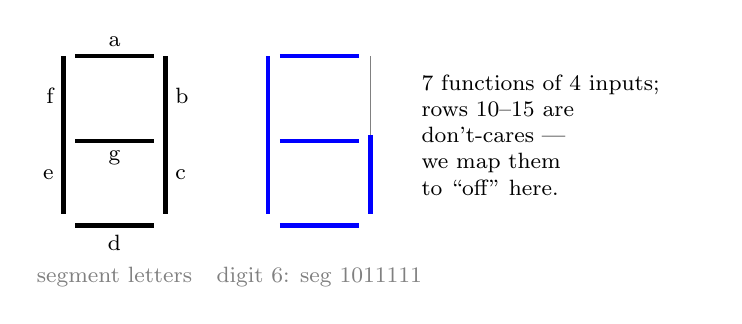
\begin{tikzpicture}[font=\footnotesize]
% segment map
\draw[ultra thick] (0,2) -- (1,2); \node[above] at (0.5,2) {a};
\draw[ultra thick] (1.15,1) -- (1.15,2); \node[right] at (1.15,1.5) {b};
\draw[ultra thick] (1.15,0) -- (1.15,1); \node[right] at (1.15,0.5) {c};
\draw[ultra thick] (0,-0.15) -- (1,-0.15); \node[below] at (0.5,-0.15) {d};
\draw[ultra thick] (-0.15,0) -- (-0.15,1); \node[left] at (-0.15,0.5) {e};
\draw[ultra thick] (-0.15,1) -- (-0.15,2); \node[left] at (-0.15,1.5) {f};
\draw[ultra thick] (0,0.92) -- (1,0.92); \node[below] at (0.5,0.92) {g};
\node[gray] at (0.5,-0.8) {segment letters};
% lit shape for digit 6 (a f g e d c on, b off)
\begin{scope}[xshift=2.6cm]
\draw[ultra thick, blue] (0,2) -- (1,2);
\draw[thin, gray] (1.15,1) -- (1.15,2);
\draw[ultra thick, blue] (1.15,0) -- (1.15,1);
\draw[ultra thick, blue] (0,-0.15) -- (1,-0.15);
\draw[ultra thick, blue] (-0.15,0) -- (-0.15,1);
\draw[ultra thick, blue] (-0.15,1) -- (-0.15,2);
\draw[ultra thick, blue] (0,0.92) -- (1,0.92);
\node[gray] at (0.5,-0.8) {digit 6: seg 1011111};
\end{scope}
% don't-care policy note
\begin{scope}[xshift=6.2cm]
\node[align=left, text width=3.6cm] at (0,1.0)
 {7 functions of 4 inputs;\\ rows 10--15 are\\ don't-cares —\\ we map them\\ to ``off'' here.};
\end{scope}
\end{tikzpicture}
